    \section{3041F: Time Series Analysis}
    \marginpar{\href{https://media.uct.ac.za/engage/theodul/ui/core.html?ltimode=true&id=b6171c7c-14c0-46a4-aa3b-9be2aa42f87f}{Time Series Video 1}}
    This course will only look at measurements that are equally spaced in time. We will not be looking at unequal spacing (ie when you measure each event as it comes).

    A time series is denoted as \(X_t, t \, \in T\) where T can be discrete or continuous.\newline
    The index \(t\) will be discrete in this course.
    \(X_t\) could be continuous, discrete, or (not in this course) qualitative. \newline \newline

    We will often plot the data, try to see if there are any patterns or trends, and then plot summary statistics which could help with forecasting.


    There are several objectives of time series analysis:
    \begin{itemize} 
        \item Description: Summarizing the data in useful ways like expectation, variance, etc.
        \item Modelling: Creating a mathematical model of the data that closely predicts what has happened.
        \item Forecasting: Using the created model to give confidence intervals and estimates for where the process will be at a specified point in the future.  Forecasting is possible through historical data, and the existance of a pattern in that data which is expected to continue into the future.
        \item Control: Deciding if a given process is beyond certain safe operating bounds or if some extra factors need to be applied to the process in order to keep it within those safe operating bounds.
    \end{itemize} 

    \marginpar{\href{https://media.uct.ac.za/engage/theodul/ui/core.html?ltimode=true&id=97be9e42-a0d6-4a54-b08e-853b4dac6c8b}{Time Series Video 2}}
    Time series are often modelled additively as a sequence of components: 
    \begin{itemize} 
        \item Trend \(\mu_t\): The underlying expectation at time \(t\) of the time series. Often modelled as a simple function.
        \item Seasonality \(s_t\): When there are repetitions in the data, with peaks and troughs.
        \item Cycles \(c_t\): which is excluded in this course.
        \item Noise \(e_t\): which represents the random fluctuations of the data.
    \end{itemize} 
    % TODO try add a matplotlib plot instead of this
    \begin{figure}[t]
        \centering
        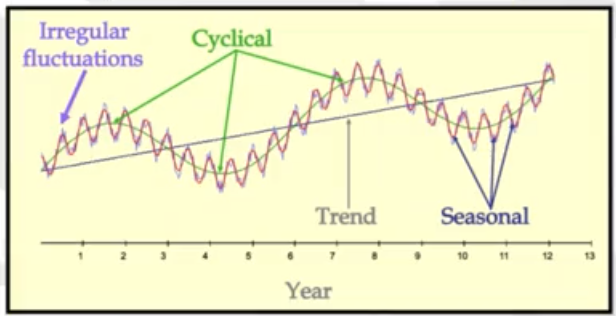
\includegraphics[width=8cm]{cycles_vs_seasons}
        \caption{Comparison of Seasons vs Cycles}
    \end{figure}

    Not every component will be included in every model.
    This can be modelled as 
    \begin{equation*}
        X_t = \mu_t + s_t + c_t + e_t
    \end{equation*}
    Or multiplicatively, although the multiplicative model will be log-transformed and then we'll just treat it as an additive model.
    \begin{equation*}
        \begin{aligned}
            X_t &= \mu_t \cdot s_t \cdot c_t \cdot e_t \\
            ln(X_t) &= ln(\mu_t) + ln(s_t) + ln(c_t) + ln(e_t) \\
        \end{aligned}
    \end{equation*}
    \subsection{Trend}
    The long term growth/decline of a time series, modelled with a simple function. Basically just the expectation.

    We can also look at the local trend, which just takes into account \(n\) prior points of the time series instead of all the data.

    Some examples of Trend:
    \begin{itemize}
        \item \(X_t = \epsilon_t\) with \(\epsilon_t \sim N(0, a)\) all iid.
            Since model's expectation \(\mu_t = \mathbb{E}[X_t] = 0\) doesn't depend on time, 
            we can use the sample mean to estimate the population mean as all samples are from the same distribution.
        \item \(X_t = t + \epsilon_t \) with \(\epsilon_t \sim N(0, a)\) all iid.
            This model's expectation \(\mu_t = \mathbb{E}[X_t] = t\) does depend on time, so the sample mean wont' be a good estimate of the true mean.
    \end{itemize}

    \subsection{Seasonality}
    When you have repeating trends in the data such as temperature increasing every summer or business flights decreasing over the weekend.

    The amplitude of the seasonality is the difference between the peaks and troughs of the data.
    This amplitude might change over time. The amplitude will affect the variance of the overall, as a high amplitude will increase the variance.

    \subsection{Cycles}
    Basically seasonality on top of the existing seasonality. If seasonality repeats every year, then cycles repeat over decades. 

    Cycles are often used to refer to less regular oscillations in the data, such as bull and bear stock market trends which are less predictable than the annual trends produced by tax deadlines and such.
    We won't be covering the cyclical component in STA3041F.

    \subsection{Transformations}
    Because of the variablity of the data, we might have to first transform the data such that our additive model is appropriate.
    Our additive model only works with data that changes linearly in time, so if the seasonality amplitude increases exponentially then we'll have to transform the data to get rid of that exponential growth.
    The family of transformations we'll be using is the Box-Cox transformations.

    \section{3041F: Transformations}
    \marginpar{\href{https://media.uct.ac.za/engage/theodul/ui/core.html?ltimode=true&id=0ab6eb00-7b9d-4895-be8a-006463cd33b0}{Time Series Video 3}}
    In figure \ref{fig:airplane_data}, you can see the seasonal component in the repeating peaks and troughs. 
    There is an upwards trend in the data and no cyclical component

    There is an increasing amount of variance as time continues as shown by how the difference between the peaks and troughs. This implies that a multiplicative model might work well.
    \begin{figure}[t]
        \centering
        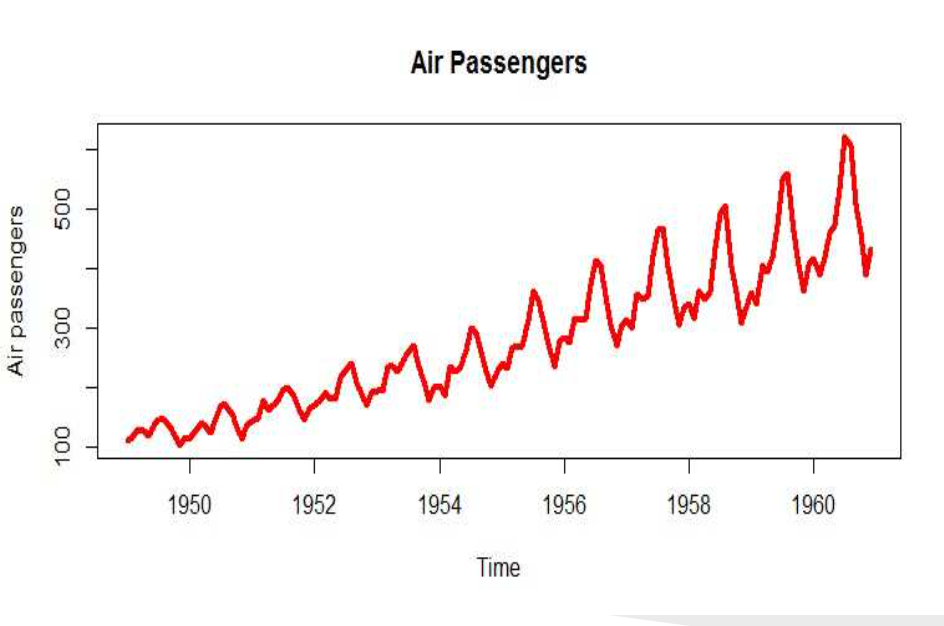
\includegraphics[width=8cm]{airplane_data}
        \caption{Airplane data}
        \label{fig:airplane_data}
    \end{figure}

    See figure \ref{fig:airplane_data_less_trend}. 
    We can now subtract the long term trend (orange) from the root data (blue) 
    in order to isolate just the error and seasonal components (assuming no 
    cyclical component):
    \begin{figure}[t]
        \centering
        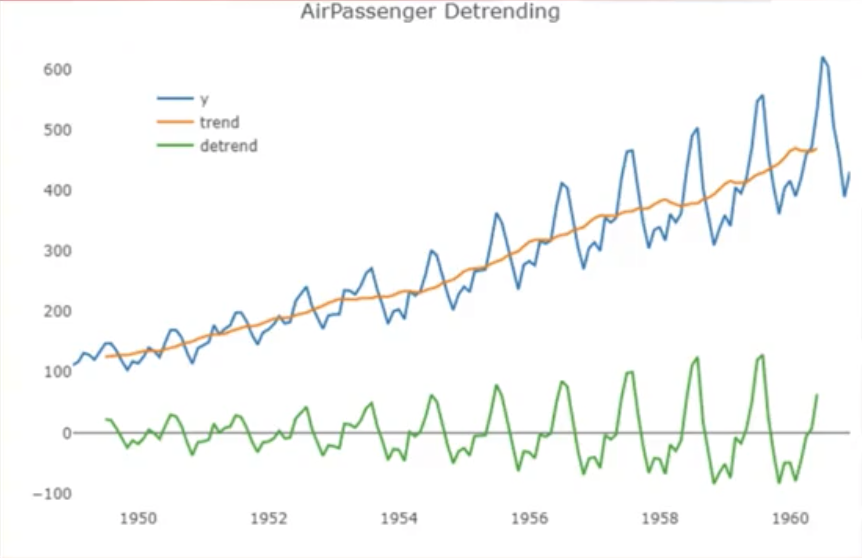
\includegraphics[width=8cm]{airplane_data_less_trend}
        \caption{Airplane data with the trend subtracted.}
        \label{fig:airplane_data_less_trend}
    \end{figure}

    Sometimes you'll want to take the root data $X_t$ and apply a transformation direcly to it
    in an attempt to end up with linear data. Transformations might also be used to make the variance equal across the series.
    Possible transformations might be $\sqrt{X_t}$, $\sqrt[3]{X_t}$, $log(X_t)$, or $-X_t^{-1}$.

    However, the Box-Cox transformation can make our lives easier:

    \subsection{3041F: Box-Cox Transformation}
    If our variance increases over time, then we want to account for this in our model. However, linear methods don't really like dealing with a changing variance. The solution is to take the original data, transform it in some way to remove/reduce how much the variance changes over time, and then proceed to use linear models on the transformed data.

    Box-Cox is a class of transformations with parameter $\lambda$  that tries to change reduce the amount the variance changes over time.

    The original series $x_1, \dots, x_n$ is transformed into $y_1(\lambda), \dots, y_n(\lambda)$ as follows:

    \begin{equation*}
        y_t(\lambda) =
        \begin{cases}
            \frac{x_t^{\lambda} - 1}{\lambda}  & \text{if $\lambda \ne 0$} \\[2ex]
            log(x_t) & \text{if $\lambda = 0$} \\
        \end{cases}
        \end{equation*}

        Where $\lambda$ has to be estimated, and the resulting transformed data has a more stabilizer variance. 
        \marginpar{\href{https://www.desmos.com/calculator/rnpu3y6lxk}{Desmos Interactive graph of the $\lambda \ne 0$ part of Box-Cox}}
        The larger value of $\lambda$, the stronger the suppressing effect of the transformation.
        Note that taking the limit as $\lambda$ trends to zero results in $log(x_t)$, which is where
        the second case of the piecewise Box-Cox comes in.
        % TODO add some matplotlib graphs showing the effect of different values of lambda

        Note that the Box-Cox tranformation is equivalent to many others, depending on the value of $\lambda$:
        \begin{itemize}
            \item When $\lambda = -1$: Inverse tranformation
            \item When $\lambda = 0$: Natural Log transformation.
            \item When $\lambda = \frac{1}{2}$: (basically) Square root transformation.
            \item When $\lambda = \frac{1}{3}$: (basically) Cube root transformation.
            \item When $\lambda = 1$: (basically) No transformation.
        \end{itemize}

        % TODO include notes on the application of Box-Cox


        \subsection{3041F: Fitting Linear Filters}
        \marginpar{\href{https://media.uct.ac.za/engage/theodul/ui/core.html?ltimode=true&id=eb6c2126-53cd-484c-a148-4cac57e904f2}{Time Series Video 4}}
        In time series analysis, we often need to remove the noise present in the data.
        Filtering the data is the processes of removing noise from the data, and there are different methods of filtering.
        \begin{figure}[t]
            \centering
            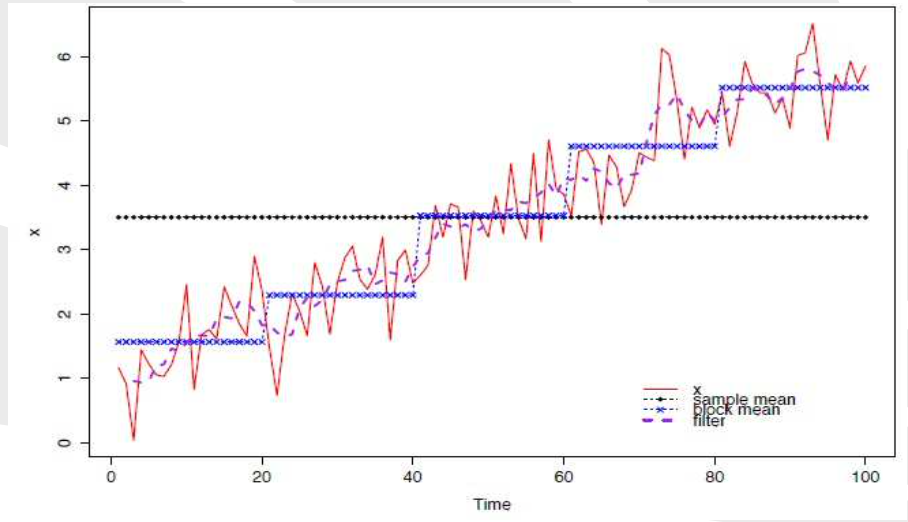
\includegraphics[width=8cm]{filtering_local_trends}
            \caption{An example of moving average, block mean, and sample mean estimates of
            the trend of the data.}
            \label{fig:filtering_local_trends}
        \end{figure}

        The sample mean of the data is often used to estimate the trend of that data. Although this assumes that the trend does not change over time (ie it's not good for increasing/decreasing data).
        An example of the sample mean is shown with the black +'s in Figure \ref{fig:filtering_local_trends}.

        A better way of estimating the trend is to divide the data into smaller blocks, and calculate the sample mean for each of those blocks. Then use these sample means to be the trend, although this still isn't great.
        An example of the block mean is shown with the blue x's in Figure \ref{fig:filtering_local_trends}.

        An even better way is via linear filters, one of which is the weighted average, an example of which is shown with the purple dashed line in Figure \ref{fig:filtering_local_trends} (labelled 'filter').

        You can see that the weighted average stays the closest to the data, while still 
        ignoring some of the jagged peaks. You can think of it as smoothing the data while
        remaining close to it.

        Linear filters can also be used to estimate seasonal components by varying various parameters that the filters take. These parameters change how smooth the filter makes the data, or how much attention it pays to local changes compared to larger scale changes.

        We can transform our original time series data $y_1, \dots, y_n$ to a filtered
        version $\tilde{y_1}, \dots, \tilde{y_n}$ by iterating over some of the items
        in $y$ and multiplying them by a weight $w$. 

        We'll look at all the $q$ items before the $y_i$ we care about, as well as all the $s$
        items after that same $y_i$. Then we'll multiply them by a weight $w_i$ and add them
        up:

        \begin{equation*}
            \tilde{y_t} = \sum_{i = -q}^{s} w_i \cdot y_{t+i}
        \end{equation*}

        Note that the $w_i$'s all have to sum to 1 (so the sample mean stays the same), 
        and usually we set $s = q$ (so we look at the same number of items behind us 
        as we do ahead of us).

        We can also show that if $\mathbb{E}[y_t] = \alpha + \beta t$ then the linear filter
        preserves this and $\mathbb{E}[\tilde{y_t}] = \alpha + \beta t$.


        The linear filter won't always preserve a quadratic trend unless we get funky with
        how we choose our weights. For example, if we have an equation for $y_t$ in the
        form:

        \begin{equation*}
            y_t = \alpha + \beta t + \phi t^2 + e_t
        \end{equation*}
        Then the expectation of our linear filter version of $y_t$ is given by
        \begin{equation*}
            \mathbb{E}[\tilde{y_t}] = \alpha + \beta t + \phi t^2 + \phi \sum_i w_i i^2
        \end{equation*}
        So in order to preserve a quadratic trend, we'd need to choose the weights $w_i$ such
        that the final term is equal to zero, ie:
        \begin{equation*}
            0 = \sum_i w_i i^2
        \end{equation*}


        Estimating the weights of the linear filter can be done as follows:
        \begin{enumerate} 
            \item Decide on how many weights you'll use. This is called the window size
            \item Decide if you're trend equation is linear, quadratic, cubic, etc.
            \item Estimate the coefficients of the trend equation $y_t = \alpha + \beta t + \dots$ using least squares.
            \item We can center the window such that the current $y_t$ is at zero, which simplifies the calculations a bit.
        \end{enumerate} 

        \paragraph{Time Series Video 5} This video was a lot of math walk-through, which I'm not going to bother writing down.
        \marginpar{\href{https://media.uct.ac.za/engage/theodul/ui/core.html?ltimode=true&id=108de531-9917-45ef-896c-90539a3e3604}{Time Series Video 5}}


        \subsection{3041F: Moving Averages}
        \marginpar{\href{https://media.uct.ac.za/engage/theodul/ui/core.html?ltimode=true&id=35c75f6e-6cf9-4e24-8a0c-1b5e9e712892}{Time Series Video 6}}
        A moving averages is a linear combination of current and past error terms.
        So we can define the moving average at time $t$ a$x_t = e_{t-n} + \dots + e_t$, 
        where we call $n$ the order of the moving average, often written as MA(n).

        There are certain useful properties, but in order for them to hold we need
        the time series to not have a seasonal component and be represented by
        \begin{equation*}
            y_t = \mu_t + e_t \qquad \text{where $\mu_t$ is the mean at time t}
        \end{equation*}
        and the error terms $e_t \sim N(0, \sigma^2)$ are all independent.
        Also, define the smoothened trend at time $t$, $\mu_t$ as:
        \begin{equation*}
            \hat{\mu}_t = \sum_{i = -s}^s w_i \cdot y_{t + i}
        \end{equation*}

        Then the following properties hold:
        \begin{equation*}
            \mathbb{V}[\hat{\mu}_t] = \sigma^2 \sum_{i = -s}^{s} w^2_i
        \end{equation*}
        \begin{equation*}
            \mathbb{C}ov[\hat{\mu}_t, \hat{\mu}_{t+k}] = 
            \sigma^2 \sum_{i = -s}^{s-k} w_i \cdot w_{i+k}
        \end{equation*}
        \begin{equation*}
            \begin{aligned}
                \mathbb{C}orr[\hat{\mu}_t, \hat{\mu}_{t+k}] &= 
                \frac{\mathbb{C}ov[\hat{\mu}_t, \hat{\mu}_{t+k}]}{
                \mathbb{V}[\hat{\mu}_t, \hat{\mu}_{t+k}]} \\
                                                            &= \frac{
                                                                \sum_{i = -s}^{s-k} w_i \cdot w_{i+k}
                                                                }{ 
                                                                \sum_{i = -s}^{s} w^2_i
                                                            }\\
                                                        \end{aligned}
    \end{equation*}

    It can also be proven that the variance of the moving average is less than the 
    variance of the original data.

    If we have a time series described by $y_t = \mu_t + e_t$ and the estimate
    for the trend is given by $\tilde{y_t}$, then we define the de-trended series
    as the difference $y_t - \tilde{y_t}$. If $\tilde{y}_t$ is an unbiased estimate
    of the trend then $\mathbb{E}[y_t - \tilde{y_t}] = 0$.

    An example of the original series and the de-trended series is shown in figure
    \ref{fig:detrended_series}

    \begin{figure}[t]
        \centering
        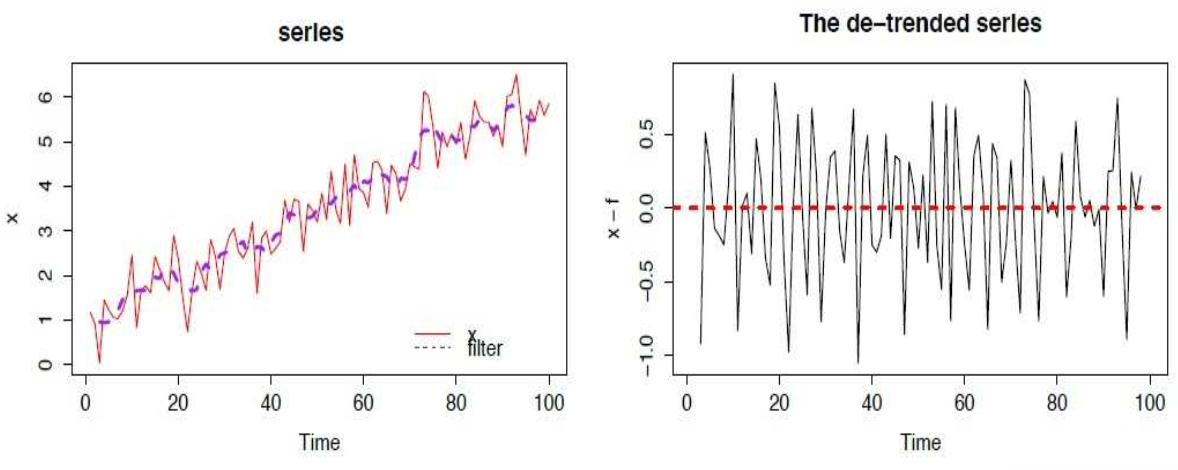
\includegraphics[width=8cm]{detrended_series}
        \caption{The detrended series has an expectation of zero if the estimate of
        the trend is unbiased.}
        \label{fig:detrended_series}
    \end{figure}

    Note that the seasonal component of a series can be removed using a moving
    average with a window size equal to the period of the season. This can be 
    seen by looking at the MA(12) line in figure \ref{fig:removing_the_seasons}


    \begin{figure}[t]
        \centering
        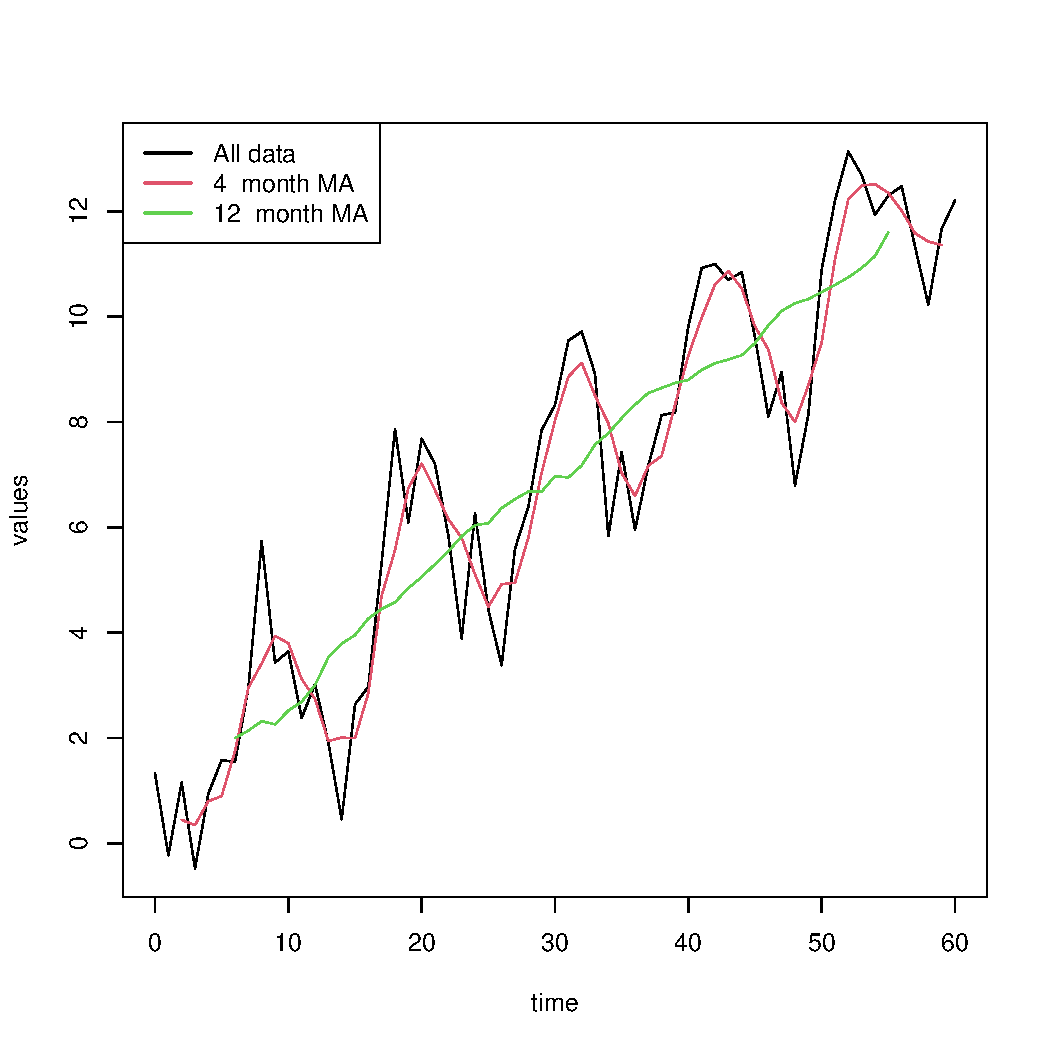
\includegraphics[width=8cm]{removing_the_seasons}
        \caption{The seasonality can be removed by applying a moving average
        which has a window size of the period of the data.}
        \label{fig:removing_the_seasons}
    \end{figure}


    Some comments about Moving Averages
    \begin{itemize} 
        \item They smoothen out a time series (ie they reduce variation) 
        \item They estimate the trend of a time series 
        \item The transformed series will be correlated with itself, as $t_i$th
            point in the moving average is a linear combination of the
            $t_{i-s}, \dots t_{i+s}$ points in the original data.  
        \item The above point means that even uncorrelated, completely random
            data will end up with correlations.  
        \item We are unable to estimate the end points, as there are no data
            points in our window
    \end{itemize} 


    \subsection{Exponential Moving Averages}
    \marginpar{\href{https://media.uct.ac.za/engage/theodul/ui/core.html?ltimode=true&id=457c7309-f3e8-402a-9ca9-924e9d3e755f}{Time Series Video 7}}
    Exponential smoothing is another type of filter. We're effectively taking
    the average but giving a higher weighting to the most recent points.  This
    filter is an asymmetric infinite filter, applying exponentially decreasing
    weights to values further back in time.

    Explicitly, the weight $w_i$ for the $i$th point in the data takes a
    parameter $0 < \alpha < 1$ and is calculated as:
    \[
        w_i = \alpha^i (1 - \alpha)
    \]
    Note that this means the sum of all weights $1 \dots \infty$ is equal to 1:
    \[
        \sum_{i=0}^\infty w_i = 1
    \]
    Single exponential smoothing is the process of using an exponentially
    weighted moving average. There are other exponential smoothing techniques,
    but we won't be looking at those.

    The exponentially smoothed value at time t ($s_t$) is given by:
    \[
        s_t = y_t(1 - \alpha) + \alpha \cdot s_{t-1}
    \]
    So the smoothed value at time $t$ depends on the smoothed value at time
    $t-1$. 
    We define the forecast for time $t+h$ as being conditional on all the
    points up to time $t$, and equal to the smoothed value $s_t$ up until that
    point:
    \begin{equation*}
        \hat{y}_{t + 1 | t} = s_t = y_t(1 - \alpha) + \alpha \cdot s_{t-1}
    \end{equation*}

    By assuming we've got an infinite number of historical values, we
    can get a closed expression for $s_t$.
    \[
    s_t = \sum_{i=0}^\infty w_i \cdot y_{t-i}
\]
    However, in the real world we don't have infinite historical values. Often
    what we do is set $s_0$ equal to the first value of the time series, and
    then all following values ($s_1, s_2, \dots$) can be calculated off of that
    starting value.

    About the value of alpha:
    \begin{enumerate}
        \item A large $\alpha$ will give lots of preference to prior values,
            leading to not very much smoothing. The weights decay very quickly.
        \item A small $\alpha$ will give lots of preference to prior values,
            leading to more smoothing. A small $\alpha$ is used for very noisy
            data.
    \end{enumerate}
    
    Basically, the choice of $\alpha$ will be chosen by trial and error,
    comparing different values according to some metric like Mean Squared
    Error, Mean Absolute Error, Sum of Squares Error, etc.


